%package list
\documentclass{article}
\usepackage[top=3cm, bottom=3cm, outer=3cm, inner=3cm]{geometry}
\usepackage{multicol}
\usepackage{graphicx}
\usepackage{url}
%\usepackage{cite}
\usepackage{hyperref}
\usepackage{array}
%\usepackage{multicol}
\newcolumntype{x}[1]{>{\centering\arraybackslash\hspace{0pt}}p{#1}}
\usepackage{natbib}
\usepackage{pdfpages}
\usepackage{multirow}
\usepackage[normalem]{ulem}
\useunder{\uline}{\ul}{}
\usepackage{svg}
\usepackage{xcolor}
\usepackage{listings}
\lstdefinestyle{ascii-tree}{
    literate={├}{|}1 {─}{--}1 {└}{+}1 
  }
\lstset{basicstyle=\ttfamily,
  showstringspaces=false,
  commentstyle=\color{red},
  keywordstyle=\color{blue}
}
%\usepackage{booktabs}
\usepackage{caption}
\usepackage{subcaption}
\usepackage{float}

\newcolumntype{M}[1]{>{\centering\arraybackslash}m{#1}}
\newcolumntype{N}{@{}m{0pt}@{}}


%%%%%%%%%%%%%%%%%%%%%%%%%%%%%%%%%%%%%%%%%%%%%%%%%%%%%%%%%%%%%%%%%%%%%%%%%%%%
%%%%%%%%%%%%%%%%%%%%%%%%%%%%%%%%%%%%%%%%%%%%%%%%%%%%%%%%%%%%%%%%%%%%%%%%%%%%
\newcommand{\itemEmail}{jmamanices@unsa.edu.pe}
\newcommand{\itemStudent}{Jhonatan Benjamin Mamani Céspedes}
\newcommand{\itemCourse}{Programación Web 2}
\newcommand{\itemCourseCode}{1702122}
\newcommand{\itemSemester}{III}
\newcommand{\itemUniversity}{Universidad Nacional de San Agustín de Arequipa}
\newcommand{\itemFaculty}{Facultad de Ingeniería de Producción y Servicios}
\newcommand{\itemDepartment}{Departamento Académico de Ingeniería de Sistemas e Informática}
\newcommand{\itemSchool}{Escuela Profesional de Ingeniería de Sistemas}
\newcommand{\itemAcademic}{2024 - A}
\newcommand{\itemInput}{Del 4 Junio 2024}
\newcommand{\itemOutput}{Al 8 Junio 2024}
\newcommand{\itemPracticeNumber}{02}
\newcommand{\itemTheme}{Vistas en Django}
%%%%%%%%%%%%%%%%%%%%%%%%%%%%%%%%%%%%%%%%%%%%%%%%%%%%%%%%%%%%%%%%%%%%%%%%%%%%
%%%%%%%%%%%%%%%%%%%%%%%%%%%%%%%%%%%%%%%%%%%%%%%%%%%%%%%%%%%%%%%%%%%%%%%%%%%%

\usepackage[english,spanish]{babel}
\usepackage[utf8]{inputenc}
\AtBeginDocument{\selectlanguage{spanish}}
\renewcommand{\figurename}{Figura}
\renewcommand{\refname}{Referencias}
\renewcommand{\tablename}{Tabla} %esto no funciona cuando se usa babel
\AtBeginDocument{%
	\renewcommand\tablename{Tabla}
}

\usepackage{fancyhdr}
\pagestyle{fancy}
\fancyhf{}
\setlength{\headheight}{30pt}
\renewcommand{\headrulewidth}{1pt}
\renewcommand{\footrulewidth}{1pt}
\fancyhead[L]{\raisebox{-0.2\height}{
\includegraphics[width=3cm]{img/logo_episunsa.png}}}
\fancyhead[C]{\fontsize{7}{7}\selectfont	\itemUniversity \\ \itemFaculty \\ \itemDepartment \\ \itemSchool \\ \textbf{\itemCourse}}
\fancyhead[R]{\raisebox{-0.2\height}{
\includegraphics[width=1.2cm]{img/logo_abet}}}
\fancyfoot[L]{Estudiante: Jhonatan Mamani}
\fancyfoot[C]{\itemCourse}
\fancyfoot[R]{Página \thepage}

% para el codigo fuente
\usepackage{listings}
\usepackage{color, colortbl}
\definecolor{dkgreen}{rgb}{0,0.6,0}
\definecolor{gray}{rgb}{0.5,0.5,0.5}
\definecolor{mauve}{rgb}{0.58,0,0.82}
\definecolor{codebackground}{rgb}{0.95, 0.95, 0.92}
\definecolor{tablebackground}{rgb}{0.8, 0, 0}

\lstset{frame=tb,
	language=bash,
	aboveskip=3mm,
	belowskip=3mm,
	showstringspaces=false,
	columns=flexible,
	basicstyle={\small\ttfamily},
	numbers=none,
	numberstyle=\tiny\color{gray},
	keywordstyle=\color{blue},
	commentstyle=\color{dkgreen},
	stringstyle=\color{mauve},
	breaklines=true,
	breakatwhitespace=true,
	tabsize=3,
	backgroundcolor= \color{codebackground},
}

\begin{document}
	
	\vspace*{10px}
	
	\begin{center}	
		\fontsize{17}{17} \textbf{ Informe de Programación Web - Django \itemPracticeNumber}
	\end{center}
	\centerline{\textbf{\Large Tema: \itemTheme}}
	%\vspace*{0.5cm}	

	\begin{flushright}
		\begin{tabular}{|M{2.5cm}|N|}
			\hline 
			\rowcolor{tablebackground}
			\color{white} \textbf{Nota}  \\
			\hline 
			     \\[30pt]
			\hline 			
		\end{tabular}
	\end{flushright}	

	\begin{table}[H]
		\begin{tabular}{|x{4.7cm}|x{4.8cm}|x{4.8cm}|}
			\hline 
			\rowcolor{tablebackground}
			\color{white} \textbf{Estudiantes} & \color{white}\textbf{Escuela}  & \color{white}\textbf{Asignatura}   \\
			\hline 
			{\itemStudent \par \itemEmail} & \itemSchool & {\itemCourse \par Semestre: \itemSemester \par Código: \itemCourseCode}     \\
			\hline 			
		\end{tabular}
	\end{table}		
	
	\begin{table}[H]
		\begin{tabular}{|x{4.7cm}|x{4.8cm}|x{4.8cm}|}
			\hline 
			\rowcolor{tablebackground}
			\color{white}\textbf{Práctica} & \color{white}\textbf{Tema}  & \color{white}\textbf{Duración}   \\
			\hline 
			\itemPracticeNumber & \itemTheme & 04 horas   \\
			\hline 
		\end{tabular}
	\end{table}
	
	\begin{table}[H]
		\begin{tabular}{|x{4.7cm}|x{4.8cm}|x{4.8cm}|}
			\hline 
			\rowcolor{tablebackground}
			\color{white}\textbf{Semestre académico} & \color{white}\textbf{Fecha de inicio}  & \color{white}\textbf{Fecha de entrega}   \\
			\hline 
			\itemAcademic & \itemInput &  \itemOutput  \\
			\hline 
		\end{tabular}
	\end{table}
	
	\section{Tarea}
	\begin{itemize}		
            \item Seguir las diapositivas de DJango02, dentro de un proyecto git local.
            \item Deberá hacer un commit por cada paso.
            \item Responder a las preguntas de las diapositivas (incluya el enunciado de la diapositiva).
            \item Incrustar la captura de pantalla al inicio de su texto de respuesta) del siguiente comando: git log --graph --pretty=oneline --abbrev-commit --all
            \item Cada commit debe ser realizado con un mensaje descriptivo del paso de la diapositiva que estuvo siguiendo.
	\end{itemize}
		
	\section{Equipos, materiales y temas utilizados}
	\begin{itemize}
            \item Sistema Operativo Windows 11 Home v 23H2 64 bits
            \item VIM x64 v9.1.
            \item Visual Studio Code x64 v1.89.1
            \item Git v2.45.0.
            \item Cuenta en GitHub con el correo institucional.
            \item Python v3.12.3.
            \item Entorno virtual.
            \item Django v5.0.6.
	\end{itemize}
	
	\section{URL de Repositorio Github}
	\begin{itemize}
            \item URL del Repositorio GitHub en donde se realiza el proyecto
            \item \url{https://github.com/JBenjamin01/pw2-django}
	\end{itemize}

    %%%%%%%%%%%%%%%%%%%% FIELD TYPES %%%%%%%%%%%%%%%%%%%%
	
    \section{Modificando el modelo Persona}

        \subsection{Cambiando los tipos de campos}
        \begin{itemize}	
            \item Como inicio de esta segunda parte del proyecto Django, se cuestiona el tipo de campo que se tenía anteriormente en el modelo Persona con charField para la edad, por esto y por la validación respecto al tamaño del campo, se modifica el modelo con tipos de datos más apropiados para sus campos.
            \item Entonces abrimos el archivo de models.py y modificamos a Persona:
            
        \begin{lstlisting}[language=bash,caption={Ingresando a models.py}][H]
        $ vim personas/models.py
        \end{lstlisting}
        \begin{lstlisting}[language=Python, caption={Modificación del modelo Persona}]
        from django.db import models
        
        # Create your models here.
        class Persona(models.Model):
            nombres = models.TextField(max_length = 100)
            apellidos = models.TextField(max_length = 100)
            edad = models.IntegerField(max_digits = 3)
        \end{lstlisting}

            \item Al haber modificado directamente el modelo Persona, necesitamos aplicar las migraciones para efectuar el cambio en la base de datos, estos generan también un nuevo archivo en migrations:
        
        \begin{lstlisting}[language=bash,caption={Makemigrations y migrate}][H]
        $ python manage.py makemigrations
        $ python manage.py migrate
        \end{lstlisting}
        
        \begin{figure}[H]
            \centering
            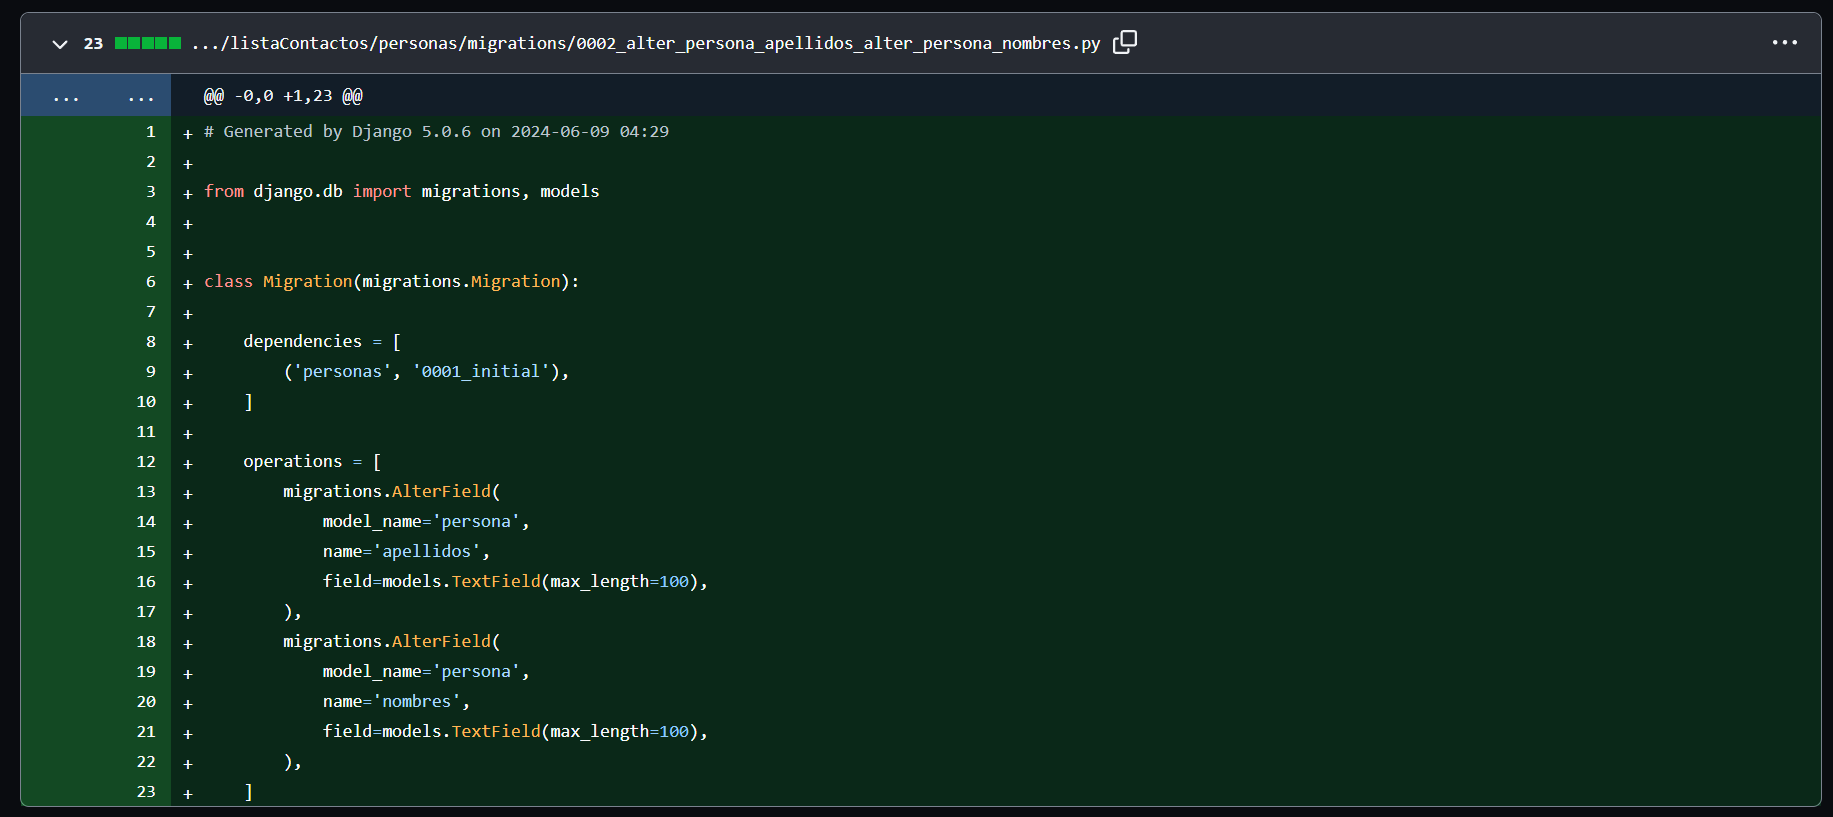
\includegraphics[width=0.7\linewidth]{img/Commit1.png}
            \caption{Archivo 0002\_alter\_persona\_apellidos\_alter\_persona\_nombres.py en GitHub}
            \label{fig:enter-label}
        \end{figure}

            \item Siguiendo las diapositivas, se crea un nuevo objeto desde el shell de Python:
        
        \begin{lstlisting}[language=bash,caption={Creación de un nuevo objeto desde el shell}][H]
        >>> from personas.models import Persona
        >>> Persona.objects.create(nombres="Jorge", apellidos="Gonzales", edad="18")
        >>> exit()
        \end{lstlisting}
            \item Posteriormente, se inicia el servidor :
        \begin{lstlisting}[language=bash,caption={Activación del servidor}][H]
        $ python manage.py runserver
        \end{lstlisting}
            \item Verificamos los cambios en el sitio de administración de Django:
        \begin{figure}[H]
            \centering
            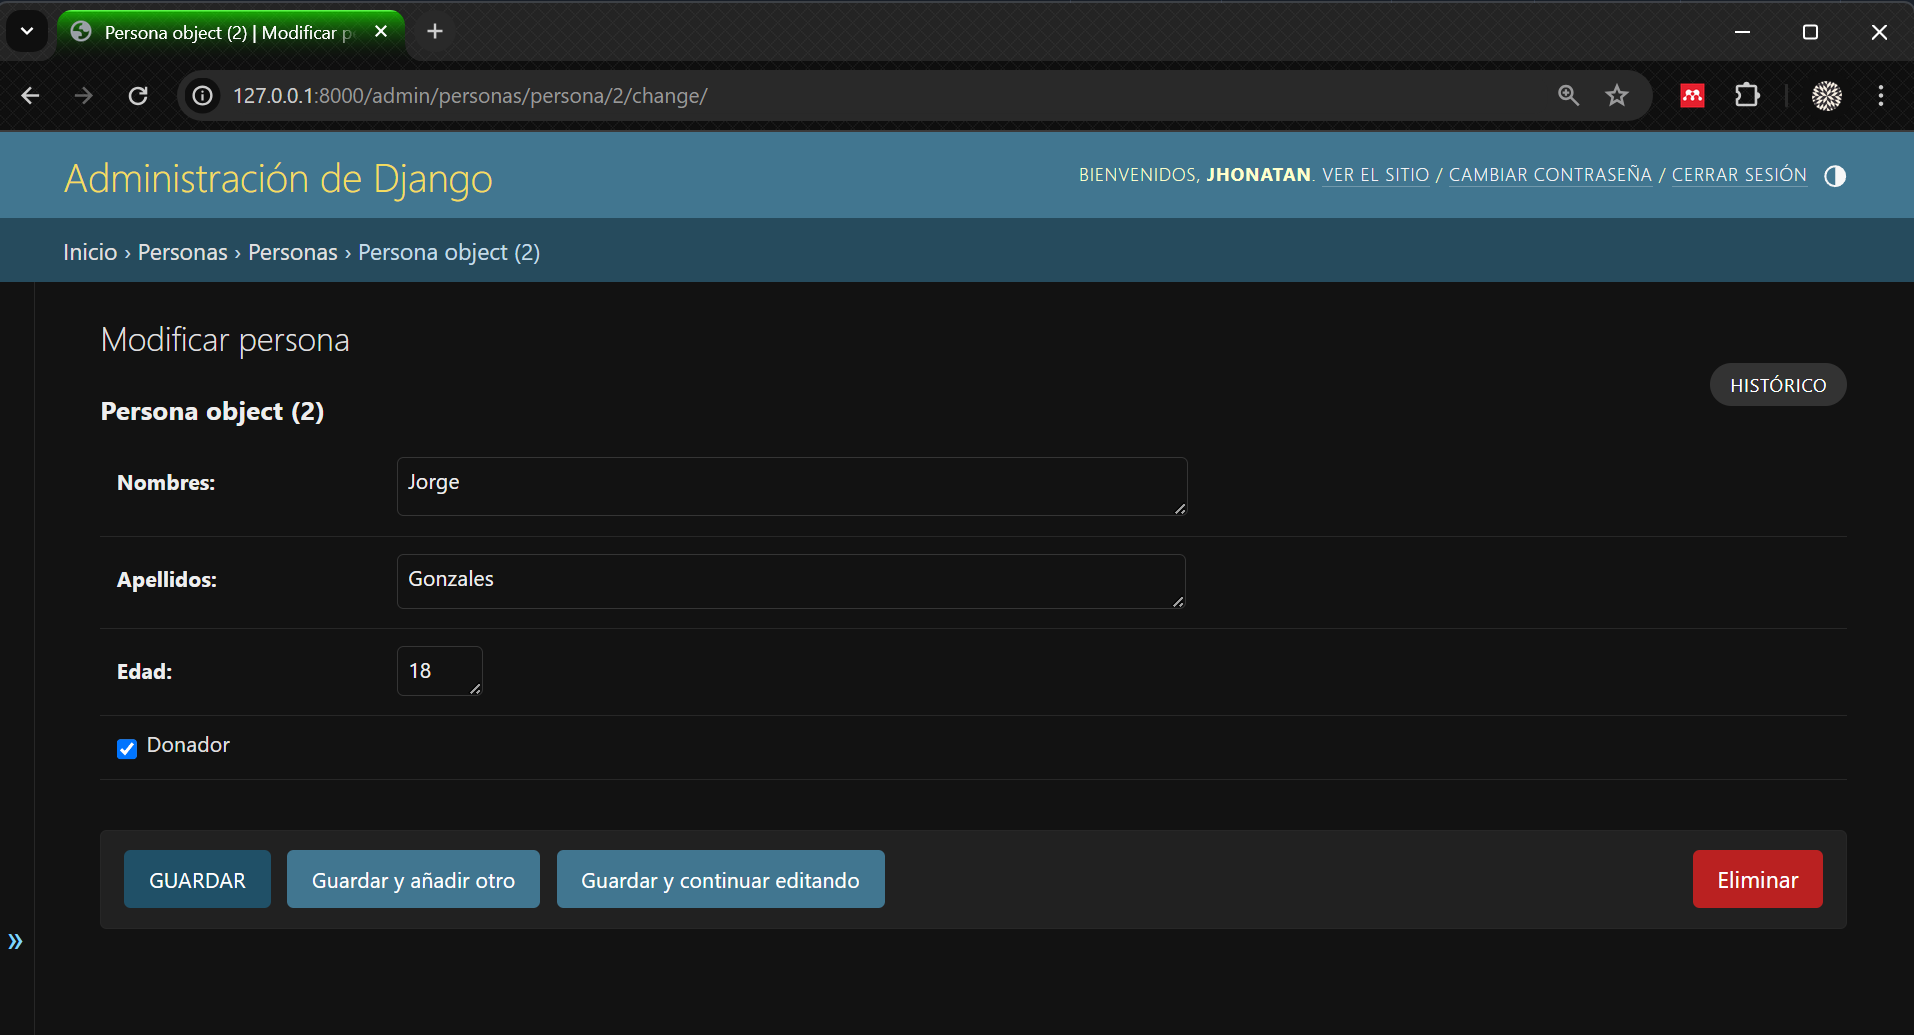
\includegraphics[width=1\linewidth]{img/Persona2.png}
            \caption{Verificación del objeto desde el Admin Site de Django}
            \label{fig:enter-label}
        \end{figure}
        \end{itemize}
        
        \subsection{Cambiando el modelo Persona (Agregando un nuevo campo)}
        \begin{itemize}
            \item Se quiere agregar un nuevo campo de tipo booleano que defina si la persona que se ingresa es donador o no, para esto se vuelve a modificar la clase Persona:
	
        \begin{lstlisting}[language=Python, caption={Modificación del modelo Persona}]
        from django.db import models
        
        # Create your models here.
        class Persona(models.Model):
            nombres = models.TextField(max_length = 100)
            apellidos = models.TextField(max_length = 100)
            edad = models.IntegerField()
            donador = models.BooleanField()
        \end{lstlisting}

            \item Al haber modificado de nuevo el modelo Persona, debemos volver a aplicar las migraciones:
        
        \begin{lstlisting}[language=bash,caption={Makemigrations}][H]
        $ python manage.py makemigrations
        \end{lstlisting}
            \item Sin embargo, antes de poder aplicarlas sale un aviso sobre el cambio que realizamos indicandonos que estamos intentando añadir un valor por defecto a las filas existentes, refiriendose a los objetos que ya habíamos creado anteriormente:

        \begin{figure}[H]
            \centering
            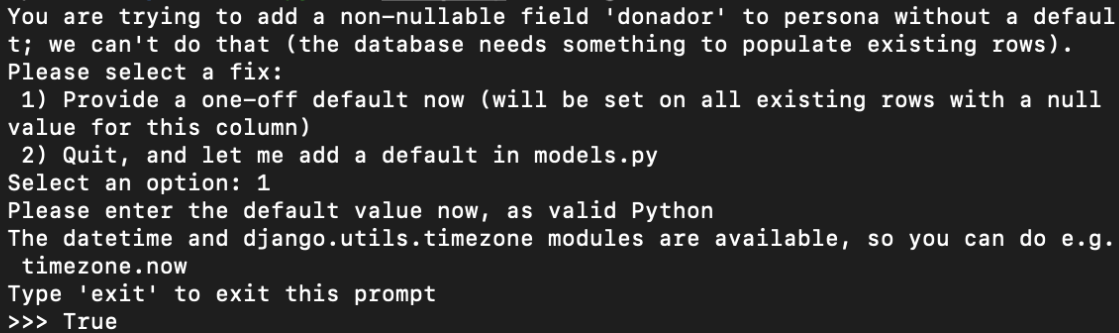
\includegraphics[width=0.8\linewidth]{img/DonadorDefault.png}
            \caption{Consola: Default para el campo donador}
            \label{fig:enter-label}
        \end{figure}
            \item Tal como se realiza en la consola de la imagen, solo seleccionamos 1 y como valor por defecto definimos a True para que todos los objetos en las filas de la base de datos se puedan actualizar correctamente:
        \begin{lstlisting}[language=bash,caption={Migrate y runserver}][H]
        $ Select an option: 1
        $ Please enter the default value now, as valid Python
        $ The datetime and django.utils.timezone modules are available, so you can do e.g.timezone.now
        $ Type 'exit' to exit this prompt
        >>> True
        \end{lstlisting}

            \item Ejecutamos el migrate e iniciamos el servidor para verificarlo:

        \begin{lstlisting}[language=bash,caption={Makemigrations y migrate}][H]
        $ python manage.py migrate
        $ python manage.py runserver
        \end{lstlisting}

            \item Observamos el primer objeto y vemos que efectivamente, ahora tiene el campo donador marcado como True pese a no haber sido creado con este valor, nuestro procedimiento fue funcional:

        \begin{figure}[H]
            \centering
            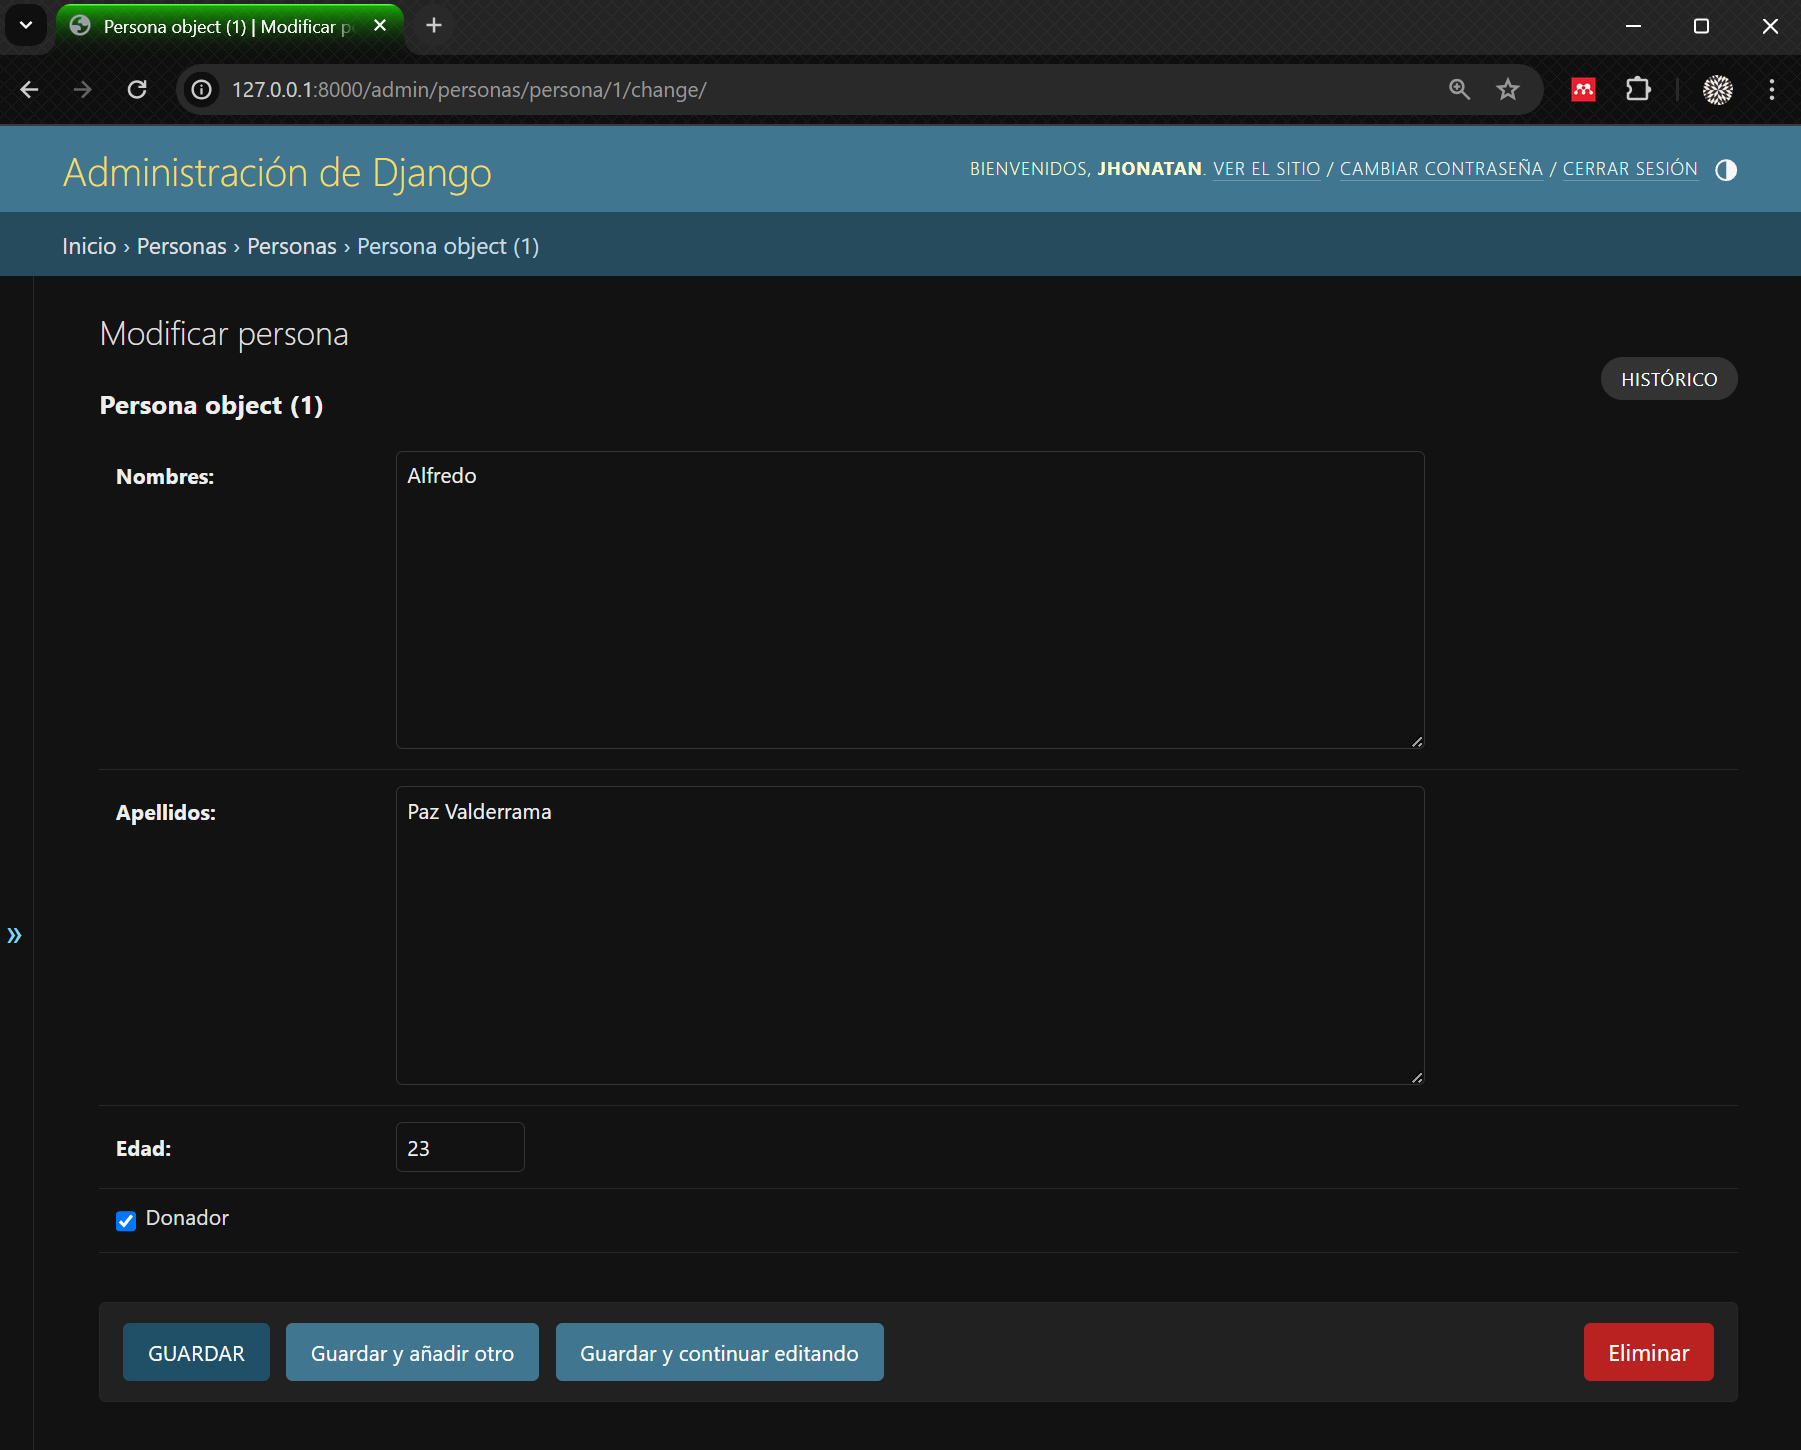
\includegraphics[width=0.7\linewidth]{img/Persona1.png}
            \caption{Objeto Persona 1}
            \label{fig:enter-label}
        \end{figure}

            \item Adicionalmente decidí implementar una forma de evitar el error con el uso de 'max\_digits = 3' para validar las entradas de las edades, en este caso, la edad puede variar entre 0 y 120:

        \begin{lstlisting}[language=Python, caption={Validación de edad}]
        from django.db import models
        from django.core.exceptions import ValidationError
        
        def validate_age(value):
            if value < 0 or value > 120:
                raise ValidationError('Edad debe estar entre 0 y 120.')
            
        # Create your models here.
        class Persona(models.Model):
            nombres = models.TextField(max_length = 100)
            apellidos = models.TextField(max_length = 100)
            edad = models.IntegerField(validators=[validate_age])
            donador = models.BooleanField()
        \end{lstlisting}
        \end{itemize}

    %%%%%%%%%%%%%%%%%%%% PÁGINA DE INICIO %%%%%%%%%%%%%%%%%%%%
    
    \section{Personalizar la página de inicio}
        \subsection{Creación de la app}
        \begin{itemize}
            \item Para modificar esta página según las diapositivas se requiere crear una clase o función en la vista de una app, es así que se decide crear una app de prueba llamada 'inicio':
             
        \begin{lstlisting}[language=bash,caption={Creación de la app inicio}][H]
        $ python manage.py startapp inicio
        \end{lstlisting}
            
            \item Tras crear esta nueva app, al igual que se había realizado anteriormente con la app 'personas', esta también se debe agregar a las apps instaladas de la configuración del proyecto, entonces nos dirigimos a settings.py:
            
        \begin{lstlisting}[language=bash,caption={Ingresando a settings.py}][H]
        $ vim listaContacto/settings.py
        \end{lstlisting}
        
            \item Bajando hasta la parte de INSTALLED\_APPS, agregamos la aplicación que acabamos de crear al final de la lista de la siguiente forma:
            
        \begin{lstlisting}[language=Python, caption={Aplicaciones del proyecto}]
        # Application definition
    
        INSTALLED_APPS = [
            'django.contrib.admin',
            'django.contrib.auth',
            'django.contrib.contenttypes',
            'django.contrib.sessions',
            'django.contrib.messages',
            'django.contrib.staticfiles',
            'personas',
            'inicio',
        ]
        \end{lstlisting}
        \subsection{Creación de la vista}
            \item Por otro lado, necesitamos crear la vista para devolver la respuesta que queremos darle a la página de inicio, por esto, modificamos el archivo de views de la aplicación recientemente creada:

        \begin{lstlisting}[language=bash,caption={Ingresando a views.py}][H]
        $ vim inicio/views.py
        \end{lstlisting}
            \item Modificamos el archivo agregando una nueva función para tener una vista sencilla que devuelve un saludo en HTML, y es un ejemplo clásico de una primera vista en un proyecto Django para asegurarse de que todo está funcionando correctamente:

        \begin{lstlisting}[language=Python, caption={Respuesta HttpResponse de la vista myHomeView}]
        from django.shortcuts import render
        from django.http import HttpResponse
        
        # Create your views here.
        def myHomeView(*args, **kwargs):
            return HttpResponse("<h1>Hola mundo desde Django</h1>")
        \end{lstlisting}
            \item El propósito de la vista myHomeView que se creó es devolver una respuesta HTTP con un mensaje "Hola mundo desde Django" incrustado en etiquetas h1. Este es un ejemplo de una vista básica que se sigue en las diapositivas, se utilizó principalmente para comprobar que el marco de trabajo está configurado correctamente y que las vistas funcionan como se espera en la página de inicio.
            
            \item El commit realizado fué el siguiente:

        \begin{figure}[H]
            \centering
            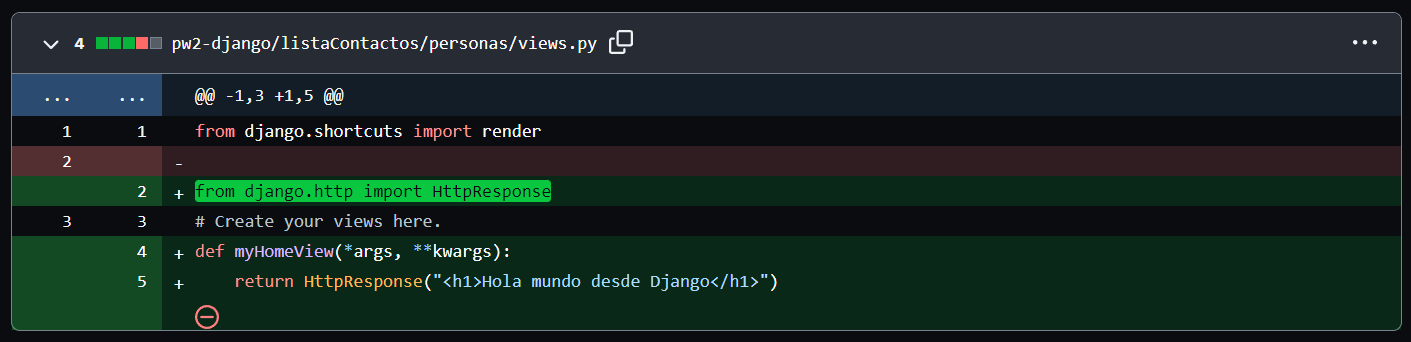
\includegraphics[width=0.8\linewidth]{img/Vista.png}
            \caption{Commit de los cambios}
            \label{fig:enter-label}
        \end{figure}
        \end{itemize}

        \subsection{Registro de la URL}
        \begin{itemize}
            \item Una vez realizada la creación de la vista, debemos registrarlo en el archivo urls.py, de esta manera podremos acceder a la página desde el servidor con el url que definamos:

        \begin{lstlisting}[language=bash,caption={Ingresando a urls.py}][H]
        $ vim inicio/urls.py
        \end{lstlisting}
            \item Con esto vamos a aseguramos de que la vista sea accesible a través de una URL en el proyecto Django, aqui se configura la URL sin especificar ingresar nada entre las comillas para que se aplique a la página de inicio:
        \begin{lstlisting}[language=Python, caption={Registro de la URL para la vista myHomeView}]
        from django.contrib import admin
        from django.urls import path
        from inicio.views import myHomeView
        
        urlpatterns = [
            path('', myHomeView, name='Pagina de Inicio'),
            path('admin/', admin.site.urls),
        ]
        \end{lstlisting}

            \item Algo interesante que se encontró aquí fué la url de admin, en donde la parte de admin.site.urls se refiere al conjunto de URLs que Django ha predefinido para el sitio de administración. Estas URLs incluyen todas las rutas necesarias para manejar la interfaz de administración, como el inicio de sesión, la página principal del admin, las páginas para agregar, editar, eliminar modelos, etc.
        
        \subsection{Verificación de la URL}
            \item Volviendo a lo que veniamos desarrollando, solo nos queda revisar que la URL de nuestra vista funcione correctamente, para esto volvemos a iniciar el servidor:

        \begin{lstlisting}[language=bash,caption={Inicio del servidor}][H]
        $ python manage.py runserver
        \end{lstlisting}

            \item Entonces, con el servidor activo, nos vamos a dirigir hacia la página de inicio principal de Django en \url{http://127.0.0.1:8000/}, aquí  encontraremos lo siguiente:
        
        \begin{figure}[H]
            \centering
            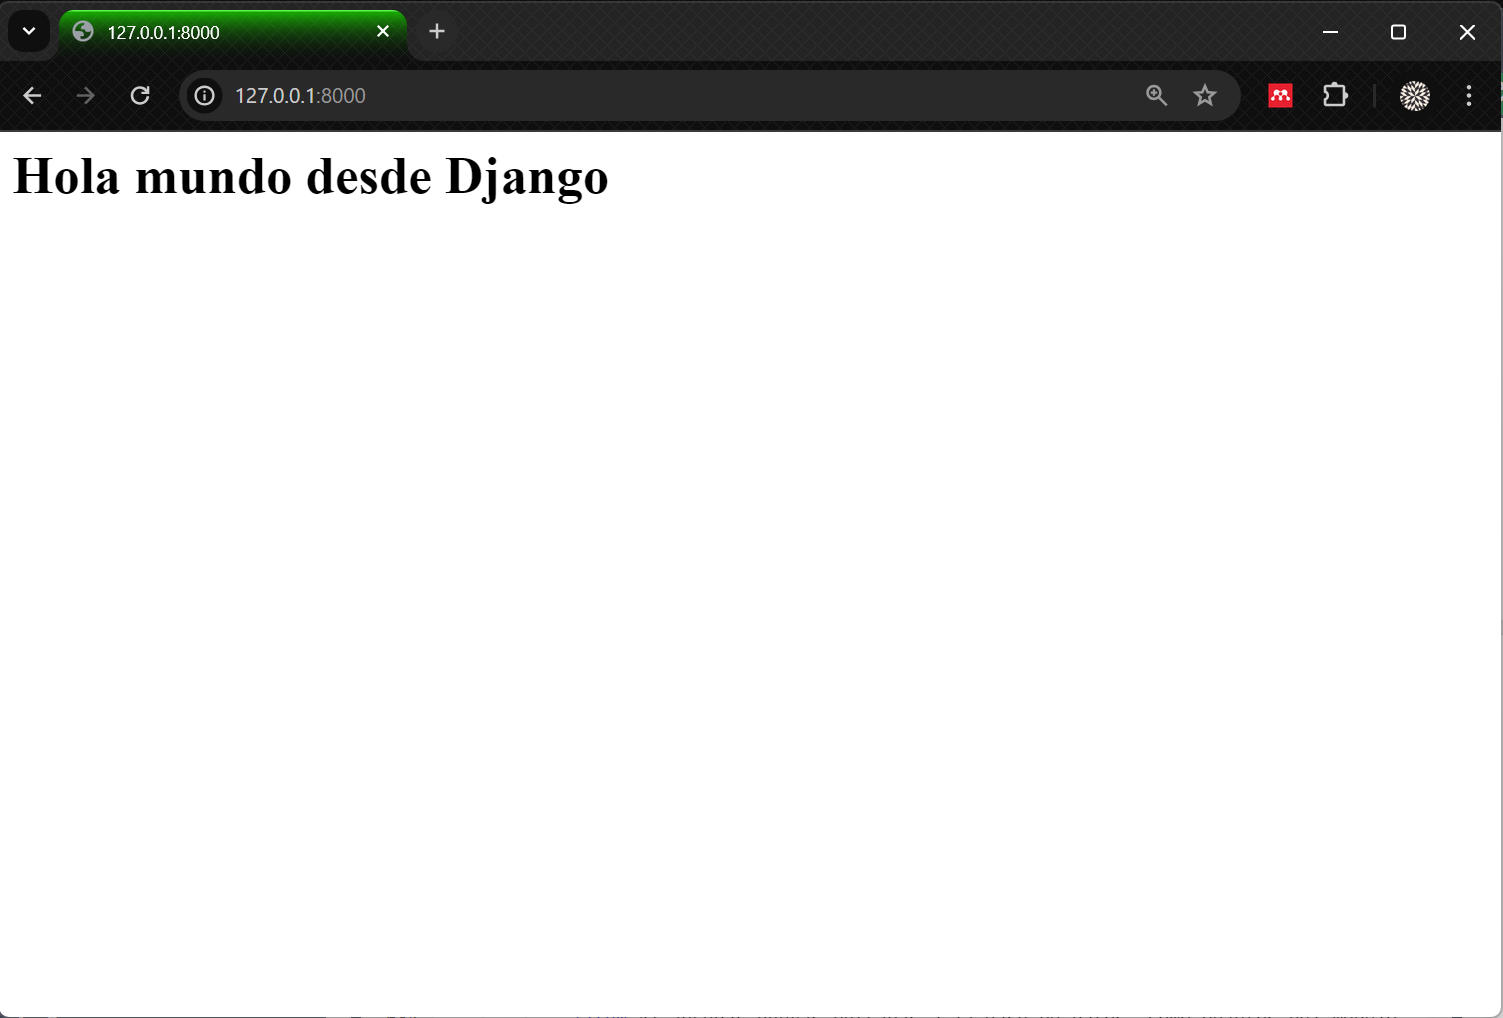
\includegraphics[width=1\linewidth]{img/Inicio.png}
            \caption{Página de Inicio con la nueva vista}
            \label{fig:enter-label}
        \end{figure}
            \item En donde comprobamos que funciona correctamente.
        \end{itemize}

    %%%%%%%%%%%%%%%%%%%% PETICIONES Y RUTEO %%%%%%%%%%%%%%%%%%%%
    
    \section{Peticiones y ruteos de URL}
        \subsection{URL}
        \begin{itemize}
            \item Definiendo un poco acerca del funcionamiento y relación entre las vistas y rutas, las vistas en Django son las que manejan peticiones HTTP y pueden responder de acuerdo con el método de la solicitud (GET, POST, etc.), en cuanto a los ruteos, el archivo urls.py mapea las URLs a las vistas correspondientes, permitiendo una navegación estructurada y lógica dentro de la aplicación según nosotros vayamos viendo convenientemente.
            \item Entonces, si decidimos crear una nueva URL para la misma vista no habría ningún problema mientras exista la vista y por lógica no tenga la misma ruta.
            \item Procedemos a abrir de nuevo el archivo de urls.py para agregar la nueva ruta:

        \begin{lstlisting}[language=bash,caption={Ingresando a urls.py}][H]
        $ vim inicio/urls.py
        \end{lstlisting}
            \item Definimos la URL adicional con una nueva cadena que mapee una ruta con el siguiente complemento al final: otro/
        
        \begin{lstlisting}[language=Python, caption={Registro de la nueva URL para la vista myHomeView}]
        from django.contrib import admin
        from django.urls import path
        from inicio.views import myHomeView
        
        urlpatterns = [
            path('', myHomeView, name='Pagina de Inicio'),
            path('otro/', myHomeView, name='Pagina de Inicio'),
            path('admin/', admin.site.urls),
        ]
        \end{lstlisting}
        
            \item Entonces, volviendo al servidor activo, si nos dirigimos a la nueva ruta \url{http://127.0.0.1:8000/otro/} se mostrará la misma vista de myHomeView:

        \begin{figure}[H]
            \centering
            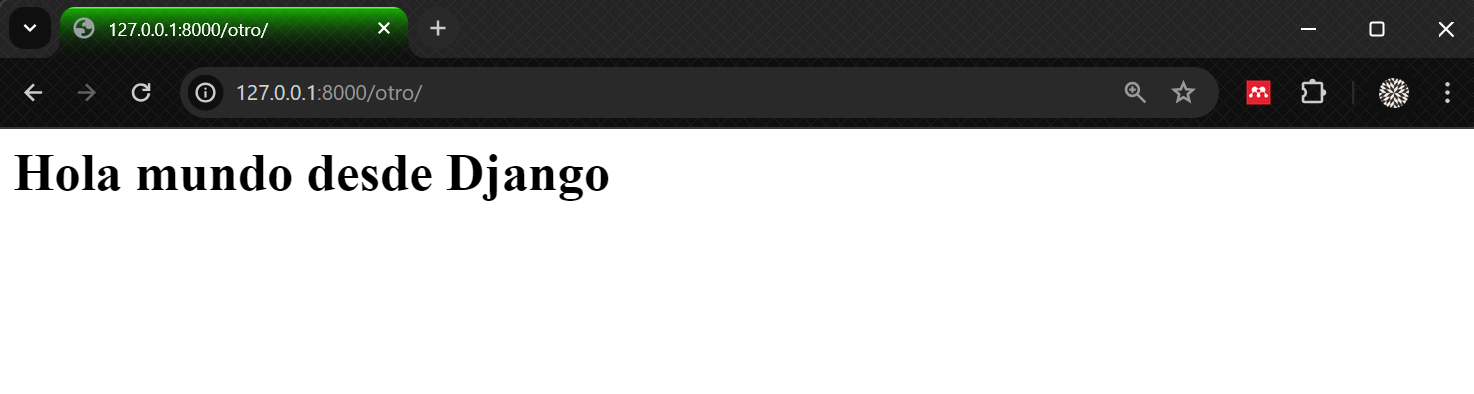
\includegraphics[width=1\linewidth]{img/URL2.png}
            \caption{Visualización en la página enrutada /otro}
            \label{fig:enter-label}
        \end{figure}
        
        \subsection{Nuevas vistas}
            \item Con lo anteriormente realizado, es posible desarrollar más vistas con diferentes lógicas de respuesta, siguiendo las diapositivas, se crea una nueva para la URL con la ruta de /otro/
            \item Nos dirigimos entonces a views.py de nuevo:

        \begin{lstlisting}[language=bash,caption={Ingresando a views.py}][H]
        $ vim inicio/views.py
        \end{lstlisting}

            \item Creamos la nueva vista anotherView:
        
        \begin{lstlisting}[language=Python, caption={Creación de la nueva vista anotherView}]
        from django.shortcuts import render
        from django.http import HttpResponse
        
        # Create your views here.
        def myHomeView(*args, **kwargs):
            return HttpResponse("<h1>Hola mundo desde Django</h1>")
        def anotherView(request):
            return HttpResponse("<h1>Solo otra pagina mas</h1>")
        \end{lstlisting}

            \item Un dato a considerar aquí es la diferencia que manejan los argumentos que reciben las dos vistas, por ejemplo, en anotherView la vista recibe un solo argumento, request, que es una instancia de HttpRequest. Según la práctica con Django parece ser el método más común y estándar para definir vistas. También encontré que el objeto request contiene toda la información sobre la solicitud HTTP actual, incluyendo datos GET y POST, cookies, y meta información.
            \item Entonces, una vez realizada esa aclaración pasamos a la ruta, nos dirigimos entonces a urls.py:

        \begin{lstlisting}[language=bash,caption={Ingresando a urls.py}][H]
        $ vim inicio/urls.py
        \end{lstlisting}
            \item Y en este archivo, asignamos la nueva vista a la segunda ruta que habíamos creado antes:
        
        \begin{lstlisting}[language=Python, caption={Asignación de la vista anotherView a la ruta /otro/}]
        from django.contrib import admin
        from django.urls import path
        from inicio.views import myHomeView
        
        urlpatterns = [
            path('', myHomeView, name='Pagina de Inicio'),
            path('otro/', anotherView),
            path('admin/', admin.site.urls),
        ]
        \end{lstlisting}
            \item Y la visualización en la página de la ruta definida ahora es la siguiente:
        \begin{figure}[H]
            \centering
            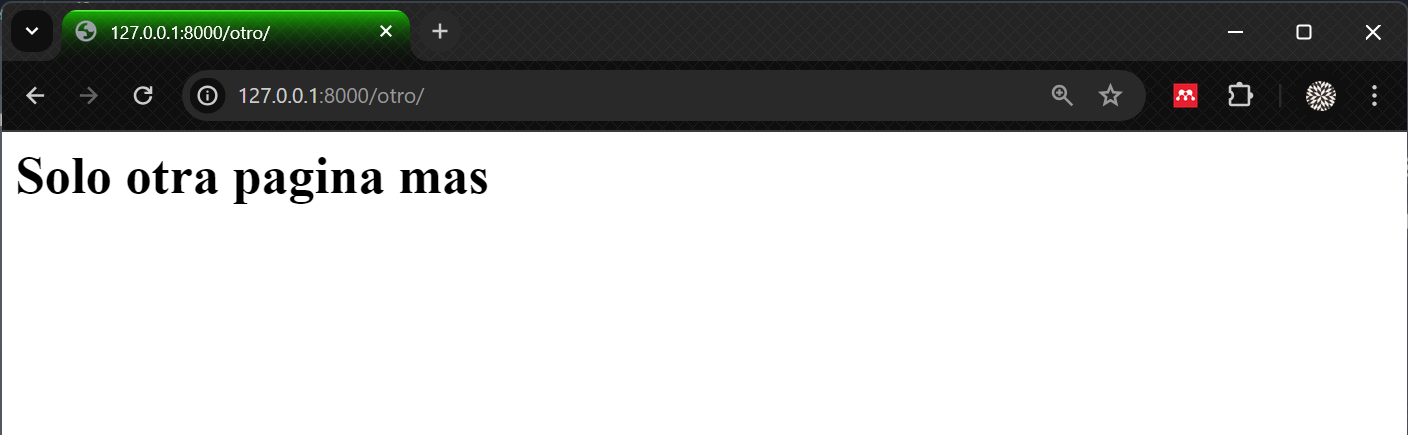
\includegraphics[width=1\linewidth]{img/Otro.png}
            \caption{Nueva vista anotherView en la ruta /otro}
            \label{fig:enter-label}
        \end{figure}
        \end{itemize}

        \subsection{Argumento de las funciones de vistas}
        \begin{itemize}
            \item Como se había visto antes, las vistas reciben argumentos diferentes, en este caso, las diapositivas buscan imprimir los argumentos además del usuario que hace la solicitud.
            \item Nos dirigimos a views.py:

        \begin{lstlisting}[language=bash,caption={Ingresando a views.py}][H]
        $ vim inicio/views.py
        \end{lstlisting}

            \item Agregamos los print para imprimir estos valores:
        
        \begin{lstlisting}[language=Python, caption={Impresión de argumentos dentro de la función}]
        from django.shortcuts import render
        from django.http import HttpResponse
        
        # Create your views here.
        def myHomeView(request, *args, **kwargs):
            print(args, kwargs)
            print(request.user)
            return HttpResponse("<h1>Hola mundo desde Django</h1>")
        def anotherView(request):
            return HttpResponse("<h1>Solo otra pagina mas</h1>")
        \end{lstlisting}

            \item Entonces, en nuestro servidor activo volveremos a ingresar a la página de inicio. Y en la consola se nos mostrará lo siguiente:

        \begin{figure}[H]
            \centering
            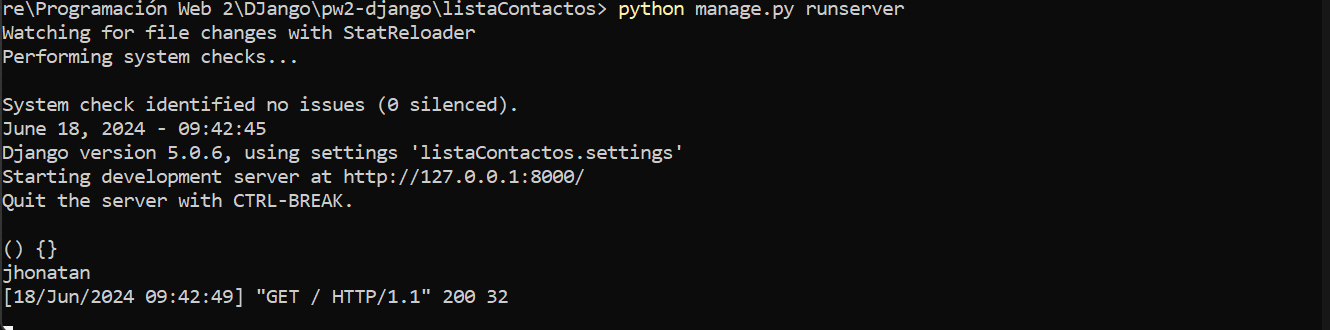
\includegraphics[width=1\linewidth]{img/Argumentos.png}
            \caption{Argumentos y usuario impresos en consola}
            \label{fig:enter-label}
        \end{figure}

            \item Como se observó, además de devolver la respuesta HTTP que muestra el mensaje "Hola mundo desde Django", dentro de la misma función, se imprimieron los valores de args y kwargs, así como el usuario que hizo la solicitud con request.user.
            \item Finalmente, si ingresamos desde el modo incógnito, la impresión del valor de usuario que realiza la solicitud cambia a anónimo:

        \begin{figure}[H]
            \centering
            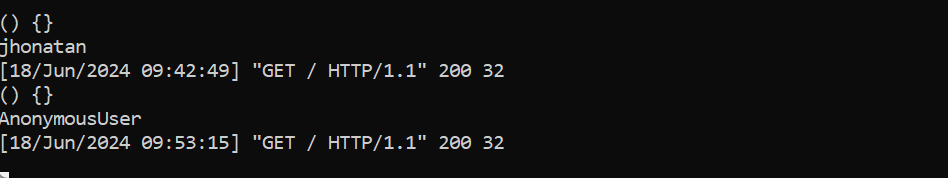
\includegraphics[width=0.8\linewidth]{img/Anonymous.png}
            \caption{Argumentos y usuario anónimo}
            \label{fig:enter-label}
        \end{figure}
        \end{itemize}
    \clearpage
    
    %%%%%%%%%%%%%%%%%%%% TEMPLATES %%%%%%%%%%%%%%%%%%%%
    
    \section{Plantillas (Templates) de Django}
        \subsection{Templates}
        \begin{itemize}
            \item Los templates son la forma que tiene Django para generar código HTML, en las diapositivas se asignan algunas funciones simplificadas de esta forma:
            \begin{itemize}
                \item URL es la ruta
                \item Views es la lógica
                \item Template es el HTML
            \end{itemize}
            \item Para diseñar nuestros primeros templates creamos un nuevo directorio:
        \begin{lstlisting}[language=bash,caption={Directorio templates}][H]
        $ mkdir templates
        \end{lstlisting}
        
            \item Creamos una nueva plantilla de HTML:
            
        \begin{lstlisting}[language=bash,caption={Creando el archivo home.html}][H]
        $ vim templates/home.html
        \end{lstlisting}

            \item Y desarrollamos la estructura de nuestro HTML básico:
            
        \begin{lstlisting}[language=HTML,caption={Contenido de home.html}][H]
        <!DOCTYPE html>
        <html>
            <head>
                <title>Template Base</title>
            </head>
            <body>
                <h1>Hola Mundo desde Django!!</h1>
                <h2>Con Templates</h2>
            </body>
        </html>
        \end{lstlisting}

            \item Configuramos los TEMPLATES del archivo settings.py del proyecto 
            
        \begin{lstlisting}[language=bash,caption={Ingresando a settings.py}][H]
        $ vim listaContactos/settings.py
        \end{lstlisting}

            \item Solo se modifica la lista de DIRS y también importamos el módulo os para que funcione:
            
        \begin{lstlisting}[language=Python,caption={Configurando templates}][H]
        import os
        TEMPLATES = [
            {
                'BACKEND': 'django.template.backends.django.DjangoTemplates',
                'DIRS': [os.path.join(BASE_DIR, 'templates')],
                'APP_DIRS': True,
                ...................
        \end{lstlisting}

            \item Por último nos dirigimos a views.py

        \begin{lstlisting}[language=bash,caption={Ingresando a views.py}][H]
        $ vim listaContactos/views.py
        \end{lstlisting}

            \item Y modificamos la respuesta de la función llamando a la plantilla HTML que acabamos de crear en templates:
            
        \begin{lstlisting}[language=bash,caption={Respuesta render del template home.html}][H]
        def myHomeView(request, *args, **kwargs):
            print(args, kwargs)
            print(request.user)
            return render(request, "home.html", {}),
        \end{lstlisting}

            \item La respuesta en la página de salida es la siguiente:

        \begin{figure}[H]
            \centering
            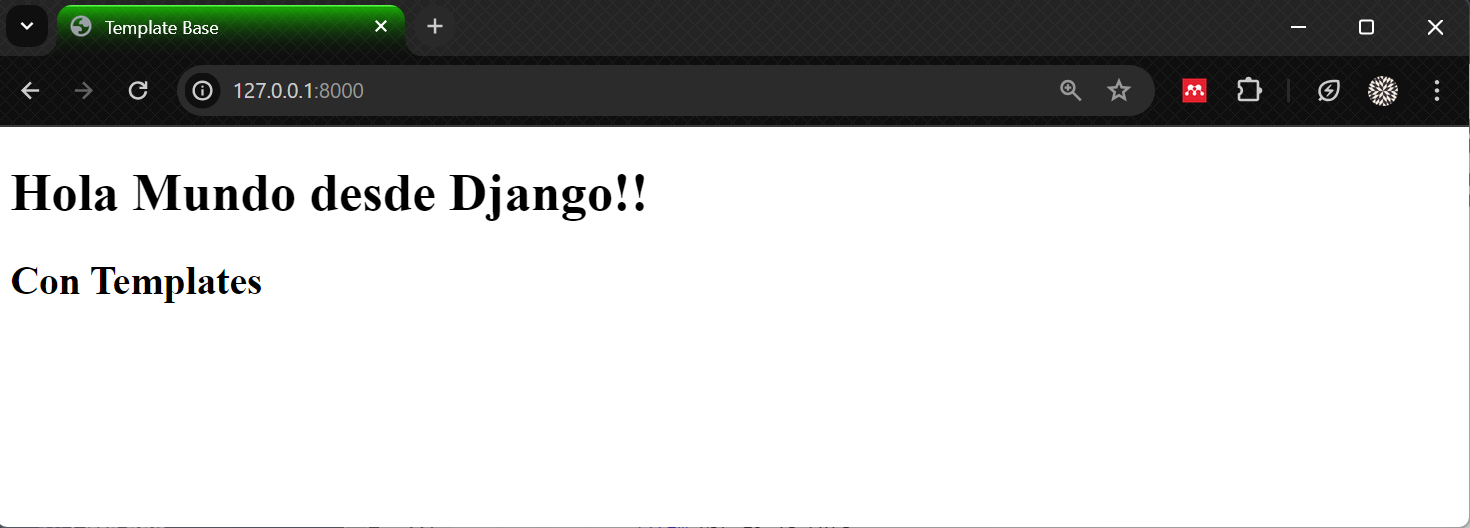
\includegraphics[width=1\linewidth]{img/Template1.png}
            \caption{Página hecha con el template home.html}
            \label{fig:enter-label}
        \end{figure}

            \item Como se ha observado, los templates son archivos HTML que pueden contener una combinación de HTML estático y sintaxis del template de Django. Estos archivos suelen almacenarse en un directorio llamado templates dentro de las aplicaciones Django.

        \subsection{Django template language (DTL): Variables}
            \item Una variable se considera como un valor según el contexto. Las variables se encuentran encerradas entre llaves dobles {{variable}}, request también puede ser usado como variable, ingresamos a la plantilla:

            \begin{lstlisting}[language=bash,caption={Ingresando a home.html}][H]
        $ vim templates/home.html
        \end{lstlisting}
    \clearpage

            \item Las variables usadas son \{\{ request.user \}\} que muestra el usuario en una pag web Django y \{\{ request.user.is\_authenticated \}\} que nos indica si está logeado.:
            
        \begin{lstlisting}[language=HTML,caption={Agregación de variables de Django}][H]
        <!DOCTYPE html>
        <html>
            <head>
                <title>Template Base</title>
            </head>
            <body>
                <h1>Hola Mundo desde Django!!</h1>
                <h2>Con Templates</h2>
                {{ request.user }}
                <br>
                {{ request.user.is_authenticated }}
            </body>
        </html>
        \end{lstlisting}
            \item La forma en la que se muestran en la página es la siguiente:
        \begin{figure}[H]
            \centering
            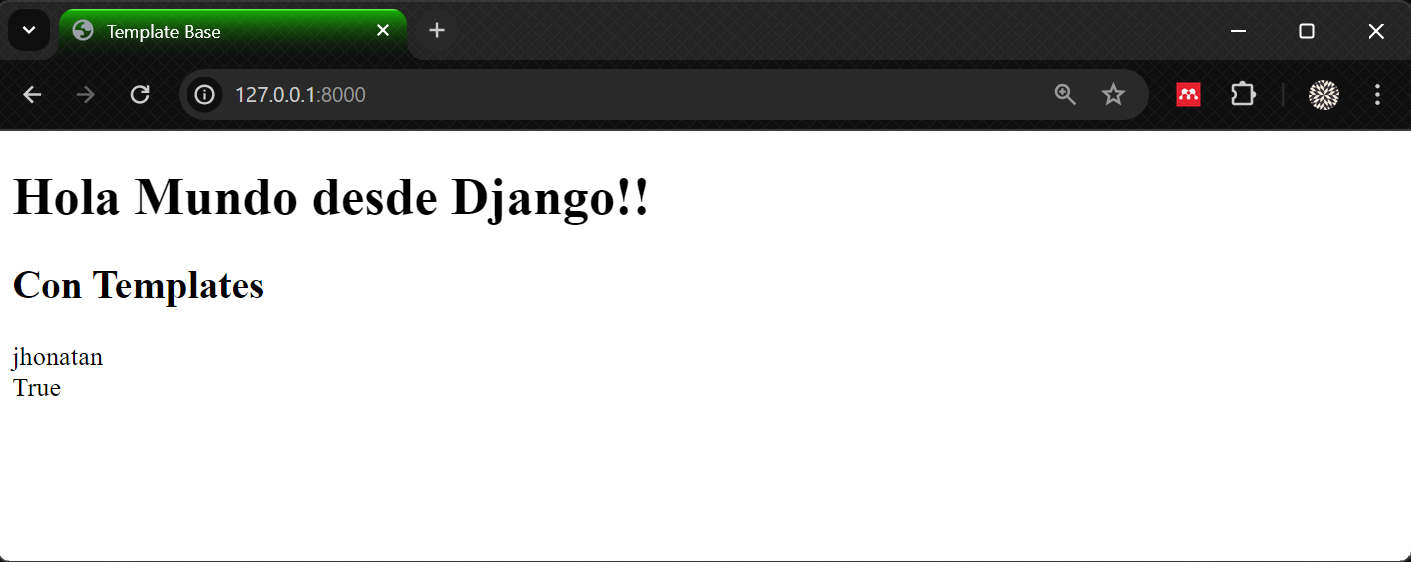
\includegraphics[width=1\linewidth]{img/Variables.png}
            \caption{Variables de request en la página principal}
            \label{fig:enter-label}
        \end{figure}
            
        \subsection{Django template language (DTL): Tags}
            \item Los tags están encerrados entre llaves con signos de porcentaje \{\% tag \%\}
            \item Pueden actuar como una estructura de control, similar a un 'if' o un bucle 'for', puede funcionar como un bloque estructural, como las llaves en lenguajes como Java, y puede usarse para extraer contenido de una base de datos o proporcionar acceso a otros tags.
            \item Para probar el uso de los tags vamos a crear un nuevo html que contendrá la plantilla base:
            
        \begin{lstlisting}[language=bash,caption={Creando la plantilla base.html}][H]
        $ vim templates/base.html
        \end{lstlisting}
        \begin{lstlisting}[language=HTML,caption={Incrustando tags block}][H]
        <!DOCTYPE html>
        <html>
            <head>
                <title>Codigo para estudiantes</title>
            </head>
            <body>
                <h1>ESTE ES UN TEXTO DE BASE</h1>
                
                    Reemplazame......
                
            </body>
        </html>
        \end{lstlisting}

        \subsection{Tag Extends}
            \item Contando con la plantilla base, se pueden definir nuevos y antiguos templates reusando algo de código, esto con el uso de extends para traer bloques de código, entramos a base.html y editamos el HTML que se usa en la vista (home.html) para que obtenga la plantilla de base.html:
        \begin{lstlisting}[language=bash,caption={Ingresando a home.html}][H]
        $ vim templates/home.html
        \end{lstlisting}
        \begin{lstlisting}[language=HTML,caption={Incrustando tag extends a la plantilla de base}][H]
        
        
        <!DOCTYPE html>
        <h2>Hola Mundo desde Django!!</h2>
        <h3>Con Templates</h3>
        {{ request.user }}
        <br>
        {{ request.user.is_authenticated }}
        
        \end{lstlisting}

            \item Si se inicia el servidor e ingresamos a la página principal nos encontramos con el código del HTML heredado de la plantilla en base.html y la información agregada de home.html:
        \begin{figure}[H]
            \centering
            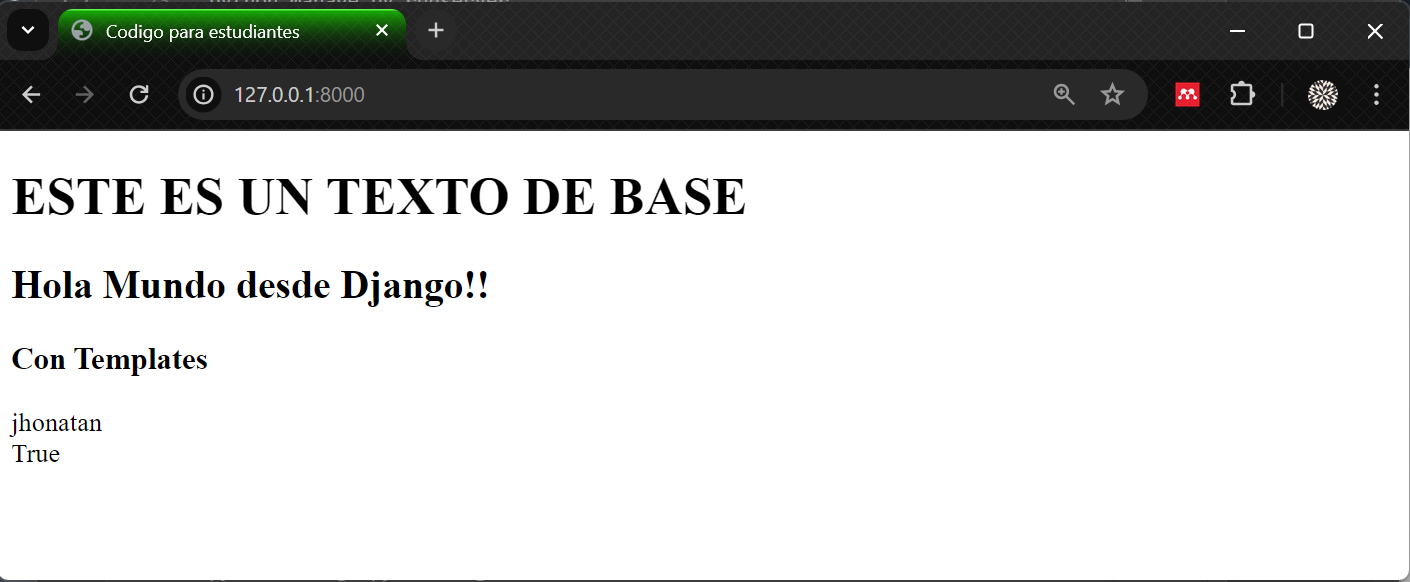
\includegraphics[width=0.7\linewidth]{img/Tag_extends.png}
            \caption{Tag extends en la página de inicio}
            \label{fig:enter-label}
        \end{figure}
        
        \subsection{Tag Include}
            \item Este tag viene a ser la manera de incrustar código de otros templates a uno nuevo.

            \item Para probarlo, se crea un nuevo html llamado nav, el cual se incrustará en base.html:
            
        \begin{lstlisting}[language=bash,caption={Creando la plantilla nav.html}][H]
        $ vim templates/nav.html
        \end{lstlisting}
            \item Definimos el contenido de nav, ya que hace referencia a un navbar, creamos una lista:
        \begin{lstlisting}[language=HTML,caption={Creando lista del navbar}][H]
        <nav>
            <ul>
                <li>Home</li>
                <li>Primero</li>
                <li>Segundo</li>
                <li>Tercero</li>
            </ul>
        </nav>
        \end{lstlisting}

        \item En base.html solo agregamos un tag include al inicio de body:
        \begin{lstlisting}[language=bash,caption={Ingresando a base.html}][H]
        $ vim templates/base.html
        \end{lstlisting}
        \begin{lstlisting}[language=HTML,caption={Incrustando el Tag include}][H]
        <body>
        
        <h1>ESTE ES UN TEXTO DE BASE</h1>
        
            Reemplazame......
        
    </body>
        \end{lstlisting}

            \item El uso de estos tags es muy útil cuando se tienen partes de HTML que se repiten en varias páginas del sitio web. En lugar de copiar y pegar el mismo código en múltiples archivos HTML, sería posible crear un template separado para esa parte y luego incluirlo en las plantillas donde lo necesites con una sola línea.
    \clearpage
            \item Finalmente, volviendo de nuevo al contenido de las diapositivas, al iniciar el servidor, en la página principal se nos muestra la lista que pusimos en el HTML de nav.html, ahora incrustado en base.html del cual extiende home.html:
        \begin{figure}[H]
            \centering
            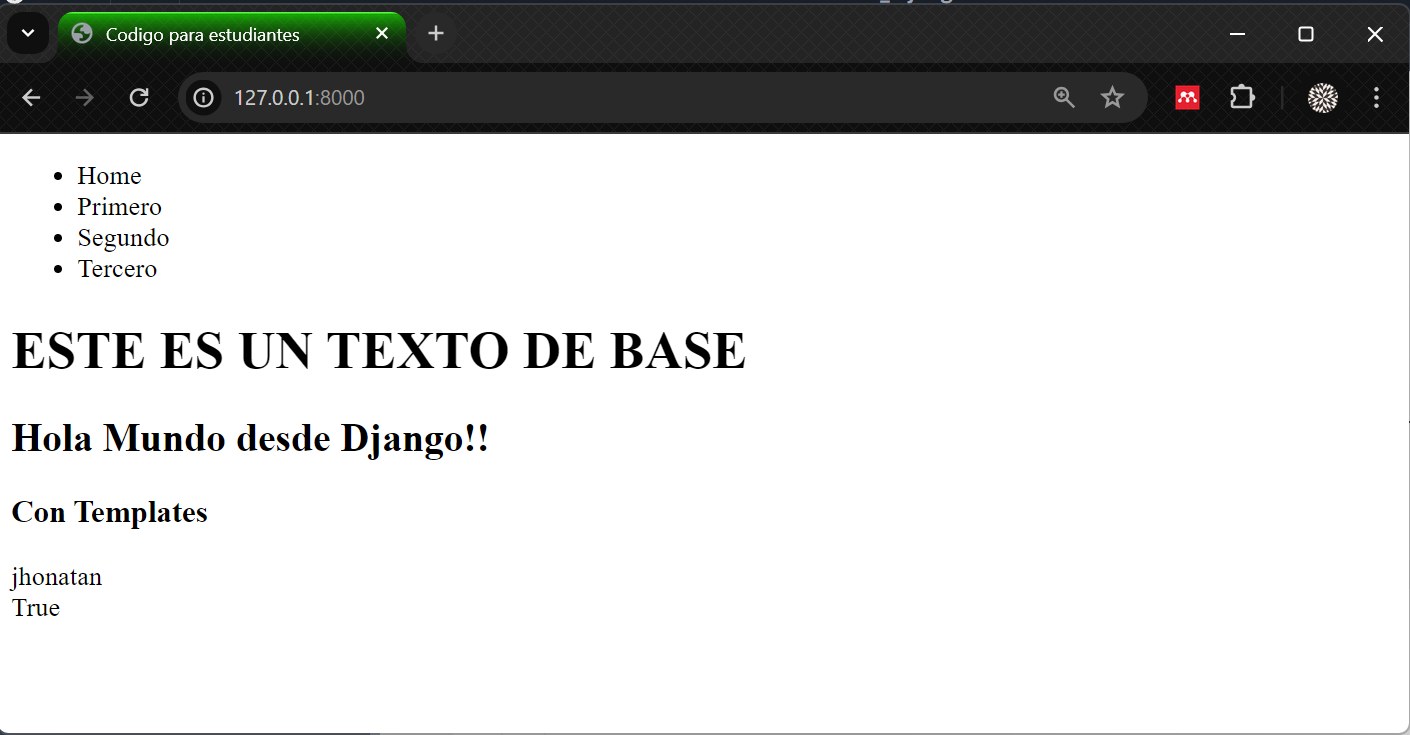
\includegraphics[width=1\linewidth]{img/Tag_include.png}
            \caption{Tag include en la página principal}
            \label{fig:enter-label}
        \end{figure}

        \end{itemize}

    \section{Captura de pantalla de commits}
        \begin{itemize}
            \item Como último paso de la actividad se ejecuta este comando para obtener el historial de los commits realizados en la actividad y le se le toma una captura, para quitar los commits anteriores, se recortaron los realizados únicamente para la diapositiva de Django 02:
        \begin{lstlisting}[language=bash,caption={Historial de commits}][H]
        $ git log --graph --pretty=oneline --abbrev-commit --all
        \end{lstlisting}
        \begin{figure}[H]
            \centering
            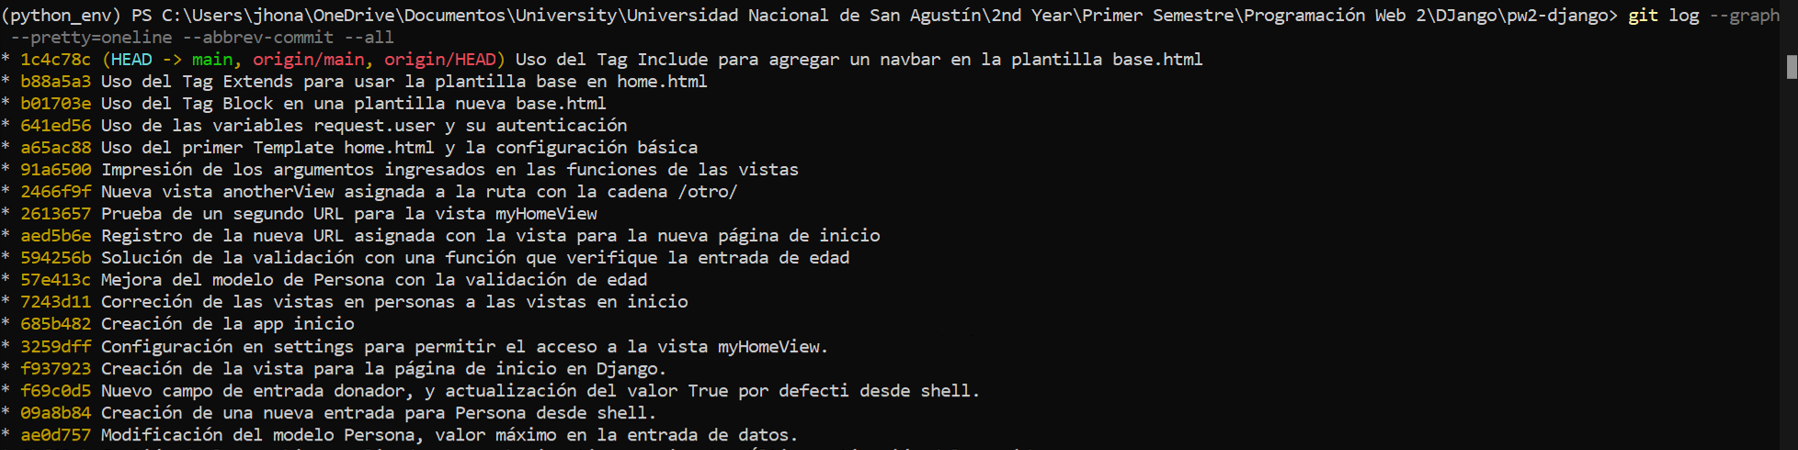
\includegraphics[width=1\linewidth]{img/Captura.png}
            \caption{Captura del historial de commits}
            \label{fig:enter-label}
        \end{figure}
        \end{itemize}
    \clearpage
    
    %%%%%%%%%%%%%%%%%%%% TREE DEL LABORATORIO %%%%%%%%%%%%%%%%%%%%
        
    \section{Estructura del trabajo}
        \begin{itemize}	
            \item El contenido que se entrega en esta práctica es el siguiente:
        \end{itemize}

        \begin{lstlisting}[style=ascii-tree]
        pw2-django/
        |--- Informe01
        |   |--- img
        |   |   |--- Admin_login.png
        |   |   |--- Admin_site.png
        |   |   |--- Admin_site2.png
        |   |   |--- Captura.png
        |   |   |--- Commmit1.png
        |   |   |--- Commmit2.png
        |   |   |--- Commmit3.png
        |   |   |--- Commmit4.png
        |   |   |--- Django_site.png
        |   |   |--- logo_abet.png
        |   |   |--- logo_episunsa.png
        |   |   |--- logo_unsa.jpg
        |   |   |--- Persona1.png
        |   |--- Informe_Django01.pdf    
        |   |--- Informe_Django01.tex
        |--- Informe02
        |   |--- img
        |   |   |--- Anonymous.png
        |   |   |--- Argumentos.png
        |   |   |--- Captura.png
        |   |   |--- Commmit1.png
        |   |   |--- DonadorDefault.png
        |   |   |--- Inicio.png
        |   |   |--- logo_abet.png
        |   |   |--- logo_episunsa.png
        |   |   |--- logo_unsa.jpg
        |   |   |--- Otro.png
        |   |   |--- Persona1.png
        |   |   |--- Persona2.png
        |   |   |--- Pregunta1.png
        |   |   |--- Pregunta2.png
        |   |   |--- Tag_extends.png
        |   |   |--- Tag_include.png
        |   |   |--- Template.png
        |   |   |--- URL2.png
        |   |   |--- Variables.png
        |   |   |--- Vista.png
        |   |--- Informe_Django02.pdf    
        |   |--- Informe_Django02.tex
        |--- pw2-django
        |   |--- listaContactos
        |   |   |--- listaContactos
        |   |   |   |---__init__.py
        |   |   |   |--- asgi.py
        |   |   |   |--- settings.py
        |   |   |   |--- urls.py
        |   |   |   |--- wsgi.py
        |   |   |--- inicio
        |   |   |   |--- migrations
        |   |   |   |   |--- __init__.py
        |   |   |   |--- __init__.py
        |   |   |   |--- admin.py
        |   |   |   |--- apps.py
        |   |   |   |--- models.py
        |   |   |   |--- tests.py
        |   |   |   |--- views.py
        |   |   |--- personas
        |   |   |   |--- migrations
        |   |   |   |   |--- 001_initial.py
        |   |   |   |   |--- 0002_alter_persona_apellidos_alter_persona_nombres.py
        |   |   |   |   |--- 0003_persona_donador.py
        |   |   |   |   |--- 0004_alter_persona_edad.py
        |   |   |   |   |--- 0005_alter_persona_edad.py
        |   |   |   |   |--- __init__.py
        |   |   |   |--- __init__.py
        |   |   |   |--- admin.py
        |   |   |   |--- apps.py
        |   |   |   |--- models.py
        |   |   |   |--- tests.py
        |   |   |   |--- views.py
        |   |   |--- templates
        |   |   |   |--- base.html
        |   |   |   |--- home.html
        |   |   |   |--- nav.html
        |   |   |--- db.sqlite3
        |   |   |--- manage.py
        |   |--- Comandos.txt
        |--- .gitignore
        |--- README.md
        \end{lstlisting}
    \clearpage
    %%%%%%%%%%%%%%%%%%%% PREGUNTAS DEL INFORME %%%%%%%%%%%%%%%%%%%%
        
    \section{Preguntas:}
        \subsection{¿Qué pasa si añadimos un nuevo campo?  los anteriores registros no lo tendrían, entonces ¿Con qué valor se actualizarán?}
        \begin{figure}[H]
            \centering
            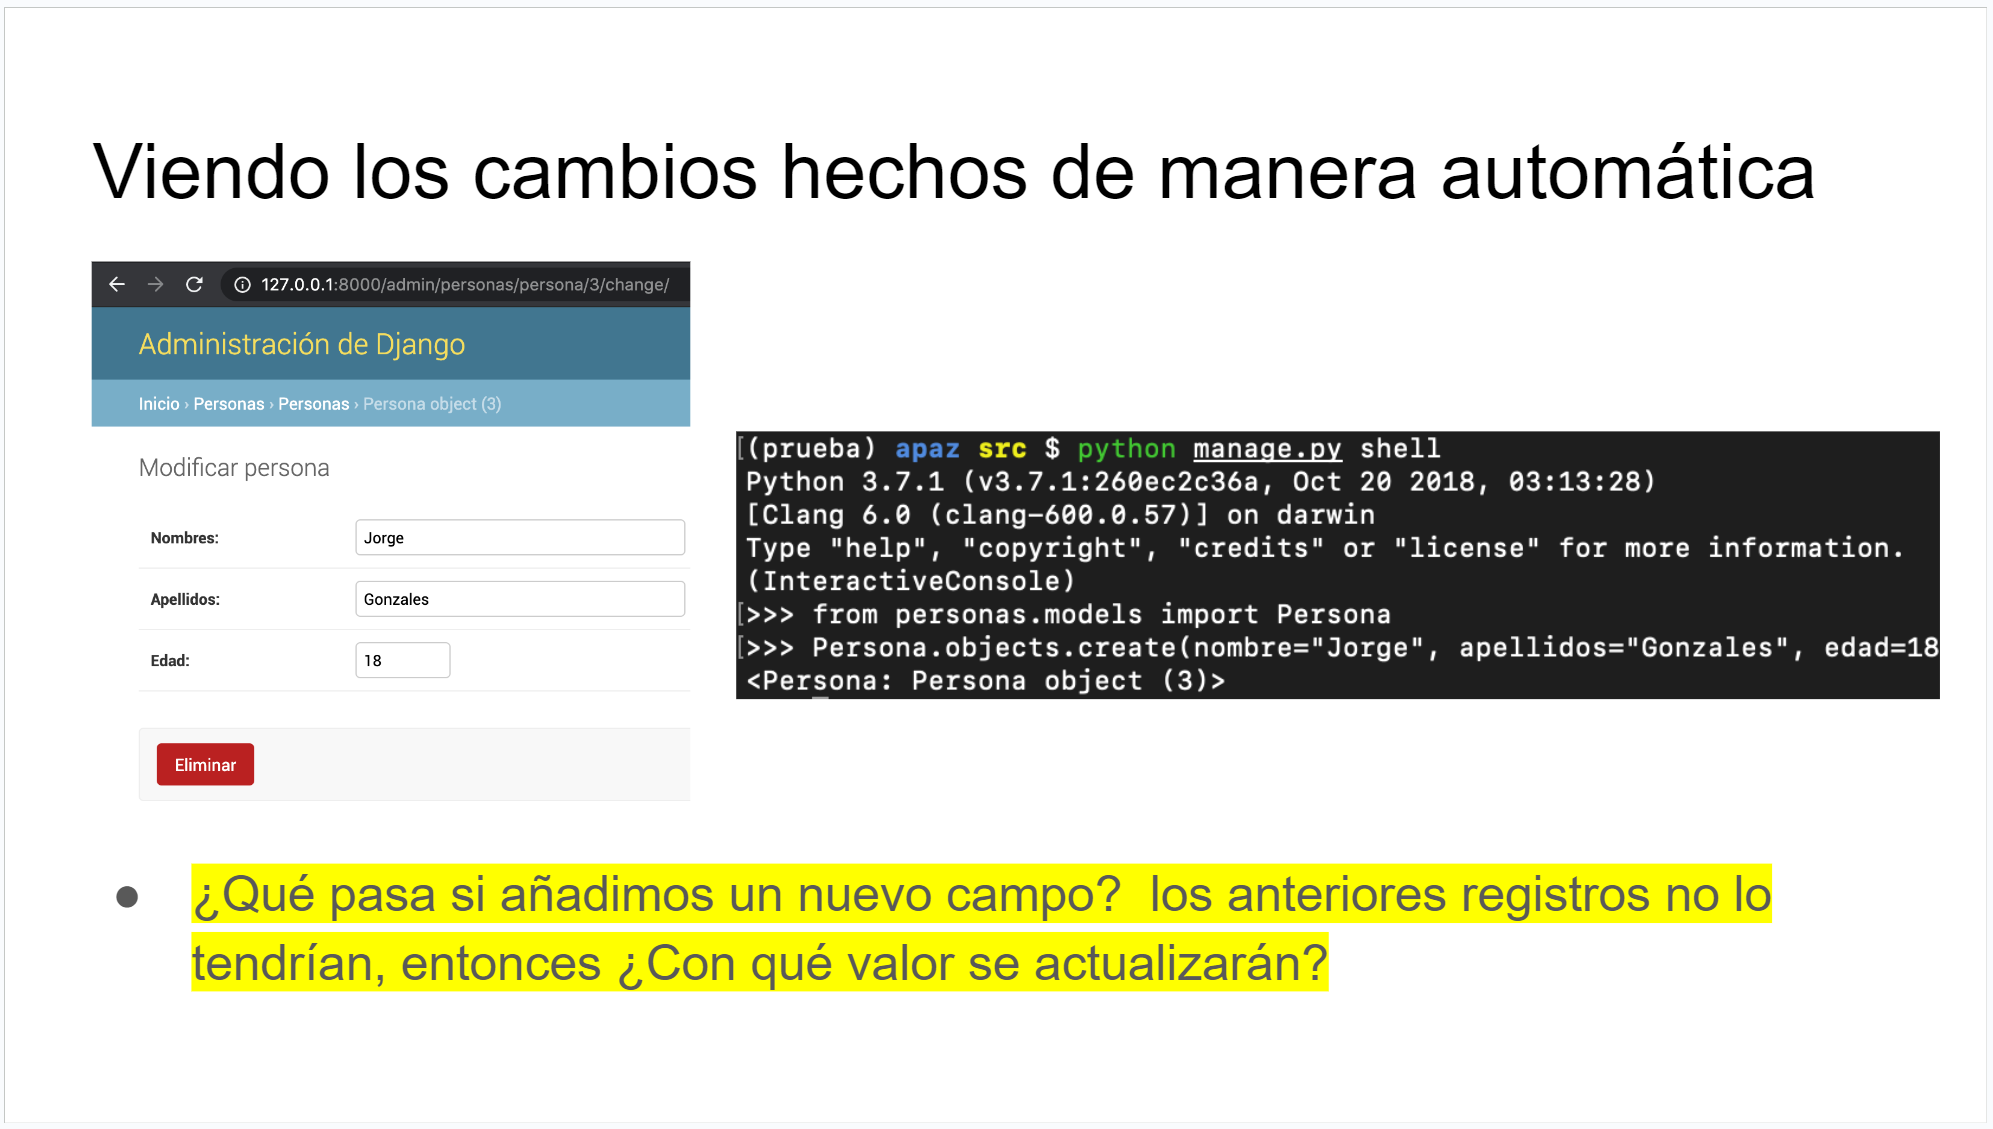
\includegraphics[width=1\linewidth]{img/Pregunta1.png}
            \caption{Captura del historial de commits}
            \label{fig:enter-label}
        \end{figure}
        \begin{itemize}
            \item Cuando añadí un nuevo campo a un modelo en Django y ejecuté makemigrations, Django creó un archivo de migración para reflejar este cambio en la base de datos; como el campo no permitía valores nulos (en mi caso, un BooleanField), me pidió un valor por defecto para asignar a los registros existentes. 
            \item Podía especificar este valor en el modelo directamente (por ejemplo, default=True) o también podía proporcionarlo durante el makemigrations. 
            \item Al ejecutar migrate, Django actualizó todos los registros existentes, asignando el valor por defecto al nuevo campo, asegurando que cada registro tuviera un valor válido y manteniendo la consistencia de la base de datos. Aquí se dió el caso:
        \begin{figure}[H]
            \centering
            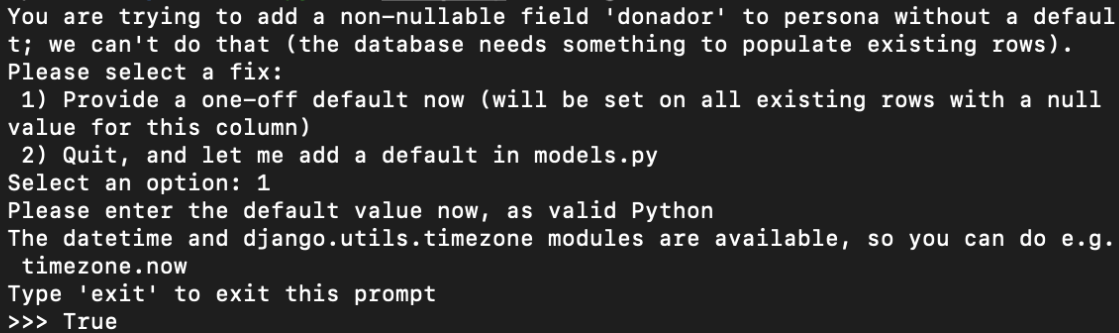
\includegraphics[width=0.8\linewidth]{img/DonadorDefault.png}
            \caption{Captura del historial de commits}
            \label{fig:enter-label}
        \end{figure}
        \end{itemize}

        \subsection{¿Cómo crearía un campo que sea obligatorio?¿Cuáles de estos elementos afectarían a la base de datos?¿Cuáles no?}
        \begin{figure}[H]
            \centering
            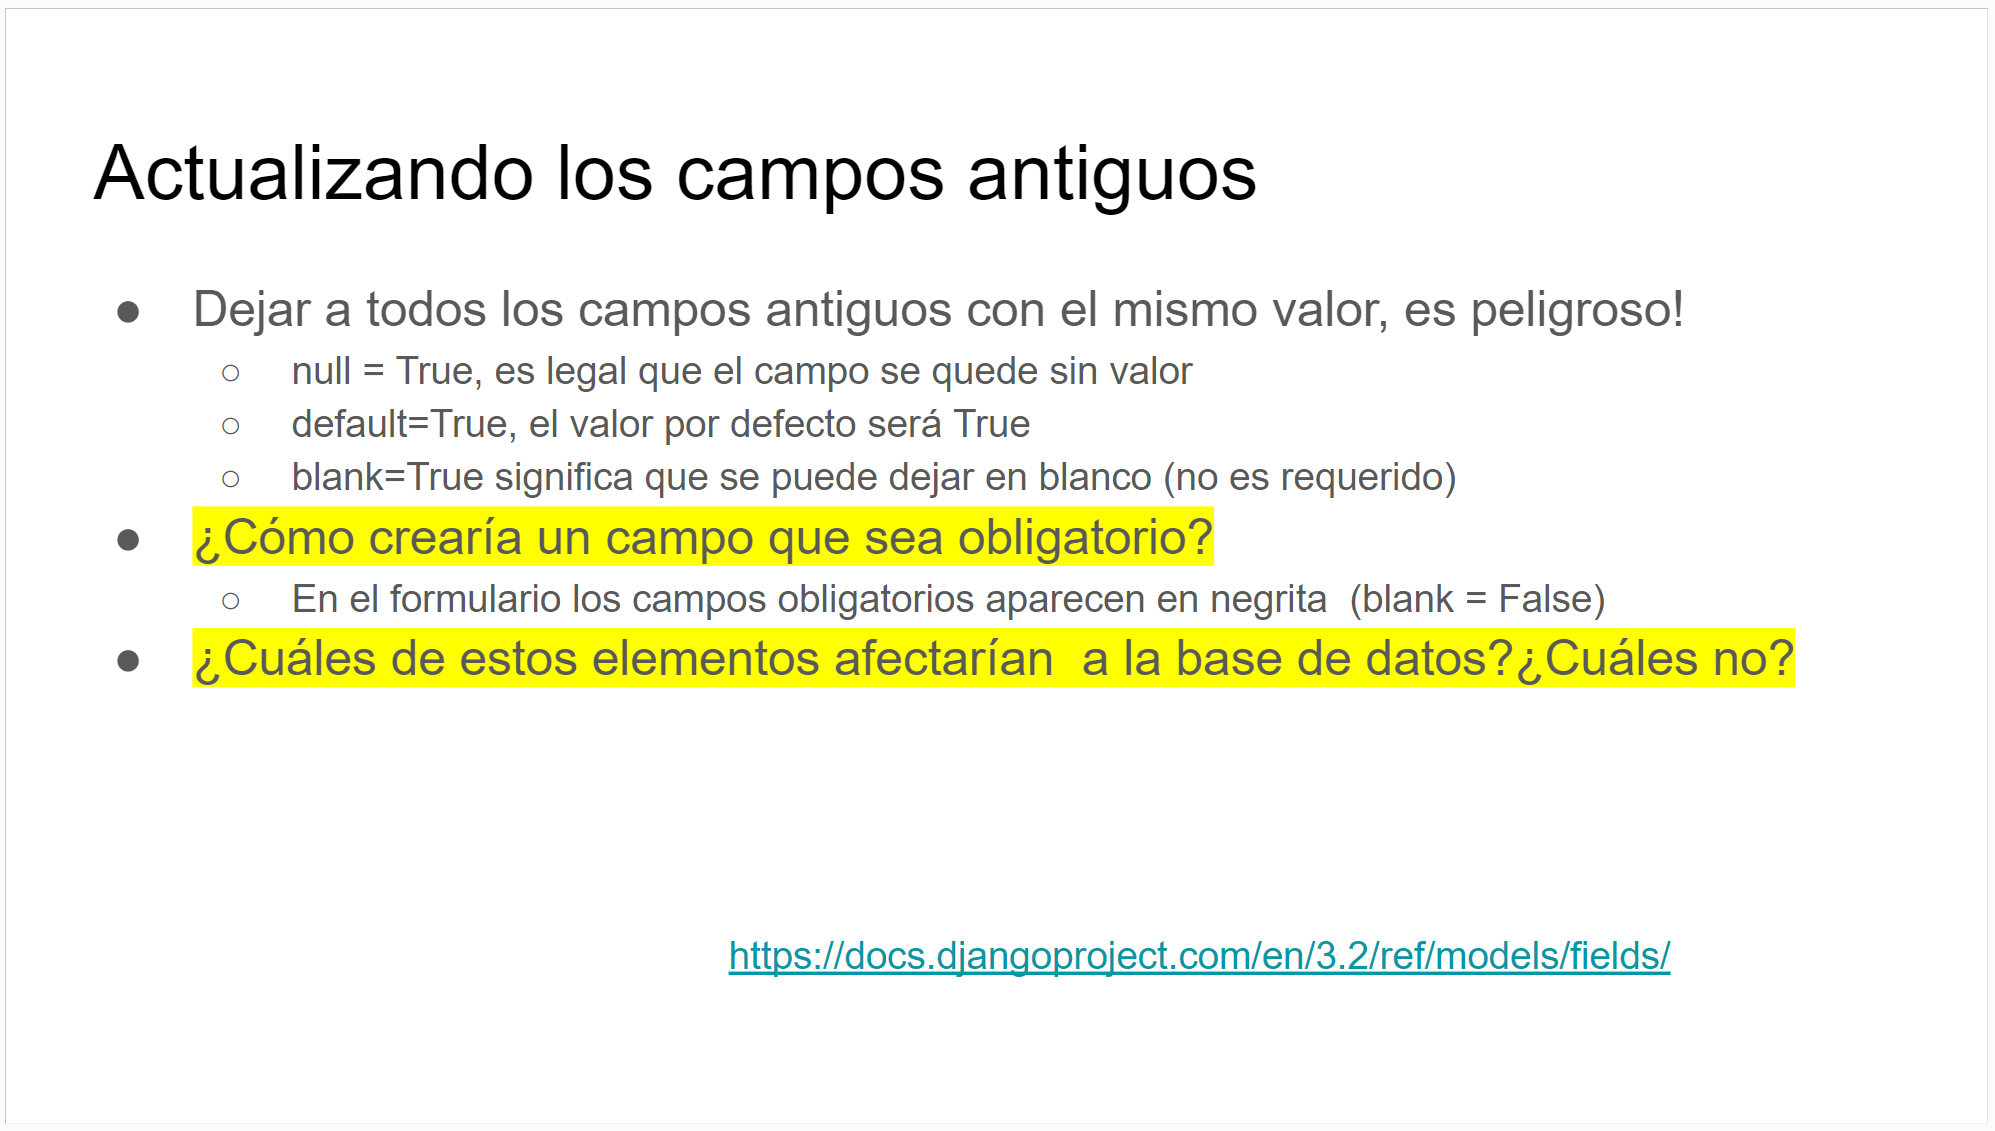
\includegraphics[width=1\linewidth]{img/Pregunta2.png}
            \caption{Captura del historial de commits}
            \label{fig:enter-label}
        \end{figure}
        \begin{itemize}	
            \item Para crear un campo obligatorio en un modelo de Django, configuro el campo con null=False y blank=False. 
            \item El parámetro null=False afecta a la base de datos porque asegura que la columna correspondiente no pueda contener valores nulos, mientras que blank=False es relevante para la validación de formularios en Django y no afecta la estructura de la base de datos. 
            \item Otros parámetros que impactan directamente la base de datos incluyen default, unique=True, y primary\_key=True, ya que estos establecen valores predeterminados, restricciones de unicidad y claves primarias, respectivamente.

        \begin{lstlisting}[language=Python,caption={Creando superusuario}][H]
        from django.db import models
        
        class Persona(models.Model):
            nombre = models.CharField(max_length=100)
            edad = models.IntegerField()
            email = models.EmailField(null=False, blank=False)  # Campo obligatorio
        \end{lstlisting}
        
            \item En contraste, aquí, los parámetros como blank=False, verbose\_name, y help\_text no afectan la estructura de la base de datos, sino que mejoran la validación y documentación en los formularios y el panel de administración de Django. 
            \item Por ejemplo, al definir un campo email en el modelo Persona con null=False, blank=False, y unique=True, garantizo que cada registro tenga un valor de email no nulo, no vacío y único, lo cual impacta tanto la base de datos como la lógica de validación en Django.
            \item Esta sería la implementación

        \begin{lstlisting}[language=Python,caption={Creando superusuario}][H]
        from django.db import models

        class Persona(models.Model):
            nombre = models.CharField(max_length=100)
            edad = models.IntegerField()
            email = models.EmailField(null=False, blank=False, unique=True, help_text="Por favor, ingrese un email valido")  # Campo obligatorio y unico
        \end{lstlisting}
        \end{itemize}

        %%%%%%%%%% RÚBRICA %%%%%%%%%%

        %\clearpage

	\section{\textcolor{red}{Rúbricas}}
	
	\subsection{\textcolor{red}{Entregable Informe}}
	\begin{table}[H]
		\caption{Tipo de Informe}
		\setlength{\tabcolsep}{0.5em} % for the horizontal padding
		{\renewcommand{\arraystretch}{1.5}% for the vertical padding
		\begin{tabular}{|p{3cm}|p{12cm}|}
			\hline
			\multicolumn{2}{|c|}{\textbf{\textcolor{red}{Informe}}}  \\
			\hline 
			\textbf{\textcolor{red}{Latex}} & \textcolor{blue}{El informe está en formato PDF desde Latex,  con un formato limpio (buena presentación) y facil de leer.}   \\ 
			\hline 	
		\end{tabular}
	}
	\end{table}
	
	\clearpage
	
	\subsection{\textcolor{red}{Rúbrica para el contenido del Informe y demostración}}
	\begin{itemize}			
		\item El alumno debe marcar o dejar en blanco en celdas de la columna \textbf{Checklist} si cumplio con el ítem correspondiente.
		\item Si un alumno supera la fecha de entrega,  su calificación será sobre la nota mínima aprobada, siempre y cuando cumpla con todos lo items.
		\item El alumno debe autocalificarse en la columna \textbf{Estudiante} de acuerdo a la siguiente tabla:
	
		\begin{table}[ht]
			\caption{Niveles de desempeño}
			\begin{center}
			\begin{tabular}{ccccc}
    			\hline
    			 & \multicolumn{4}{c}{Nivel}\\
    			\cline{1-5}
    			\textbf{Puntos} & Insatisfactorio 25\%& En Proceso 50\% & Satisfactorio 75\% & Sobresaliente 100\%\\
    			\textbf{2.0}&0.5&1.0&1.5&2.0\\
    			\textbf{4.0}&1.0&2.0&3.0&4.0\\
    		\hline
			\end{tabular}
		\end{center}
	\end{table}
	\end{itemize}
	
	\begin{table}[H]
		\caption{Rúbrica para contenido del Informe y demostración}
		\setlength{\tabcolsep}{0.5em} % for the horizontal padding
		{\renewcommand{\arraystretch}{1.5}% for the vertical padding
		%\begin{center}
		\begin{tabular}{|p{2.7cm}|p{7cm}|x{1.3cm}|p{1.2cm}|p{1.5cm}|p{1.1cm}|}
			\hline
    		\multicolumn{2}{|c|}{Contenido y demostración} & Puntos & Checklist & Estudiante & Profesor\\
			\hline
			\textbf{1. GitHub} & Hay enlace URL activo del directorio para el  laboratorio hacia su repositorio GitHub con código fuente terminado y fácil de revisar. &2 &X &2 & \\ 
			\hline
			\textbf{2. Commits} &  Hay capturas de pantalla de los commits más importantes con sus explicaciones detalladas. (El profesor puede preguntar para refrendar calificación). &4 & X& 3& \\ 
			\hline 
			\textbf{3. Código fuente} &  Hay porciones de código fuente importantes con numeración y explicaciones detalladas de sus funciones. &2 &X &2 & \\ 
			\hline 
			\textbf{4. Ejecución} & Se incluyen ejecuciones/pruebas del código fuente  explicadas gradualmente. &2 &X &2 & \\ 
			\hline			
			\textbf{5. Pregunta} & Se responde con completitud a la pregunta formulada en la tarea.  (El profesor puede preguntar para refrendar calificación).  &2 &X &2 & \\ 
			\hline	
			\textbf{6. Fechas} & Las fechas de modificación del código fuente estan dentro de los plazos de fecha de entrega establecidos. &2 &X &2 & \\ 
			\hline 
			\textbf{7. Ortografía} & El documento no muestra errores ortográficos. &2 &X &2 & \\ 
			\hline 
			\textbf{8. Madurez} & El Informe muestra de manera general una evolución de la madurez del código fuente,  explicaciones puntuales pero precisas y un acabado impecable.   (El profesor puede preguntar para refrendar calificación).  &4 & X& 4& \\ 
			\hline
			\multicolumn{2}{|c|}{\textbf{Total}} &20 & &19 & \\ 
			\hline
		\end{tabular}
		%\end{center}
		%\label{tab:multicol}
		}
        \end{table}
	
\clearpage

\section{Referencias}
\begin{itemize}			
        \item \url{https://www.w3schools.com/django/}
        \item \url{https://docs.djangoproject.com/es/5.0/intro/tutorial01/}
        \item \url{https://github.com/mdn/django-locallibrary-tutorial/blob/main/.gitignore}
        \item \url{https://developer.mozilla.org/en-US/docs/Learn/Server-side/Django/development_environment}
        \item \url{https://tutorial.djangogirls.org/es/django_views/}
        \item \url{https://www.w3schools.com/django/django_template_tags.php}
\end{itemize}	
	
%\clearpage
%\bibliographystyle{apalike}
%\bibliographystyle{IEEEtranN}
%\bibliography{bibliography}
			
\end{document}